\section{\label{I-A-1}La représentation nationale : un musée aux collections uniques}

\subsection{La lente construction du \mae}

L'histoire du \acf{mae}\footnote{Voir la chronologie de l'histoire du musée en annexe \ref{Ax-A}.} est celle d'un projet persistant, sans cesse reporté et modifié, qui trouve ses racines dans les aspirations d'associations ou de personnalités liées à l'aéronautique dès la fin du XIXe siècle\footcite{terrierAeroportParisBourget2019}. Aujourd'hui encore, il ne cesse d'évoluer : l'année 2025 a vu, outre des modernisations logicielles majeures, l'inauguration d'un nouvel espace d'exposition permanente valorisant la tour de contrôle de l'aéroport historique du Bourget\footcite{museedelairetdelespaceHallNavigationAerienne2025}.

C'est dans ces locaux que le musée s'est installé en 1973, après une longue période de recherches pour une implantation pérenne. Confronté aux aléas du XXe siècle, aux contraintes de conservation d'objets techniques et aux hésitations ministérielles, il doit sa concrétisation à l'engagement de militaires, de passionnés et à sa vocation de vitrine d'un savoir-faire français.

La décision devient effective après la Première Guerre mondiale, premier conflit à reconnaître l'importance stratégique de l'aviation. À l'initiative d'Albert Caquot, un conservatoire de l'aéronautique est confié au capitaine Hirschauer : quelques aéronefs trouvent refuge à Issy-les-Moulineaux, avant d'être déplacés à Chalais-Meudon à la suite d'une crue de la Seine. Le musée est officiellement inauguré le 23 novembre 1921 : l'institution naît, mais sans réel ancrage territorial.

Pendant l'entre-deux-guerres, il tente d'autres implantations, notamment boulevard Victor à Paris. Ces locaux, ouverts en 1936, ferment trois ans plus tard à l'aube de la Seconde Guerre mondiale. Bombardements et saisies allemandes interrompent son élan ; à la Libération, le musée réintègre Chalais-Meudon, mais demeure fermé au public durant plus de quinze ans.

S'ensuit une errance institutionnelle et territoriale : vingt-et-un sites sont envisagés entre 1952 et 1972\footcite{terrierAeroportParisBourget2019}. En 1961, le musée rouvre à Meudon, mais provisoirement. Le « Palais de l'Air et de l'Espace » poursuit sa quête de locaux adaptés à la monumentalité de ses collections. En 1973, l'ancien aéroport du Bourget, libéré au profit d'Orly, est retenu comme implantation définitive.

Dès son ouverture, le musée affirme un lien fort avec l’État et l’industrie aéronautique : le Concorde 001 lui est offert. Les collections sont progressivement transférées, Chalais-Meudon ferme en 1981, la direction rejoint le Bourget, de nouveaux halls sont ouverts au fil de l’extension du site. En 1983, à l’occasion d’un nouveau hall spatial, le musée prend son nom actuel : \acf{mae}.

Cette consolidation s’accompagne de son intégration au réseau des musées techniques : ouverture du Planétarium (1985), création de réserves à Dugny, informatisation. Fin des années 1990 : mise en place de Micromusée pour les collections, et du \ac{sigb} Alexandrie pour la bibliothèque. En 2016, l’e-médiathèque est lancée pour les fonds audiovisuels. Le \mae qui est labellisé « Musée de France » depuis 2002, se professionnalise.

Aujourd’hui, il poursuit sa modernisation : renouvellement des outils de gestion, nouveaux espaces de conservation et d’exposition. Son intégration au réseau du Grand Paris Express laisse espérer un surcroît de fréquentation. Le \mae est ainsi un musée né de ses collections, et non d’un site, dédié à la mémoire du ciel.

\subsection{Une institution complexe qui fait référence}

C’est à partir des années 1980 que le musée se structure véritablement, sous l’effet conjoint d’une reconnaissance de l’importance culturelle de l’aéronautique, d’un renouveau muséographique et de son inscription dans les réseaux nationaux. Son installation au Bourget incarne sa double fonction : conservatoire historique et vitrine stratégique. Premier aérodrome civil parisien\footcite{terrierAeroportParisBourget2019}, ce lieu symbolique ancre le musée dans la géographie et l’histoire de l’aviation française. Son lien avec le \ac{siae}, qu’il accueille tous les deux ans, renforce sa fonction promotionnelle, entre tradition et innovation.

Ce qui distingue avant tout le Musée de l’Air et de l’Espace, c’est la richesse et l’hétérogénéité de ses collections, sans équivalent national. On y trouve des aéronefs, moteurs, équipements techniques — objets exigeant des conditions de conservation particulières et une expertise rare. Cette spécificité impose des pratiques adaptées et des vocabulaires spécialisés. Mais le musée ne s’y limite pas : maquettes, estampes, objets d’art, uniformes, et, plus récemment, objets civils — vêtements, vaisselle, jouets — reflètent une évolution vers une muséographie anthropologique. Cette inflexion est incarnée notamment par la création d'un département des collections artistiques et anthropologiques, et la diversité des objets conservés se retrouve dans le schéma ci-dessous qui rassemble les différents noms de domaines des collections du musée.

\begin{figure}[htbp]
	\centering
	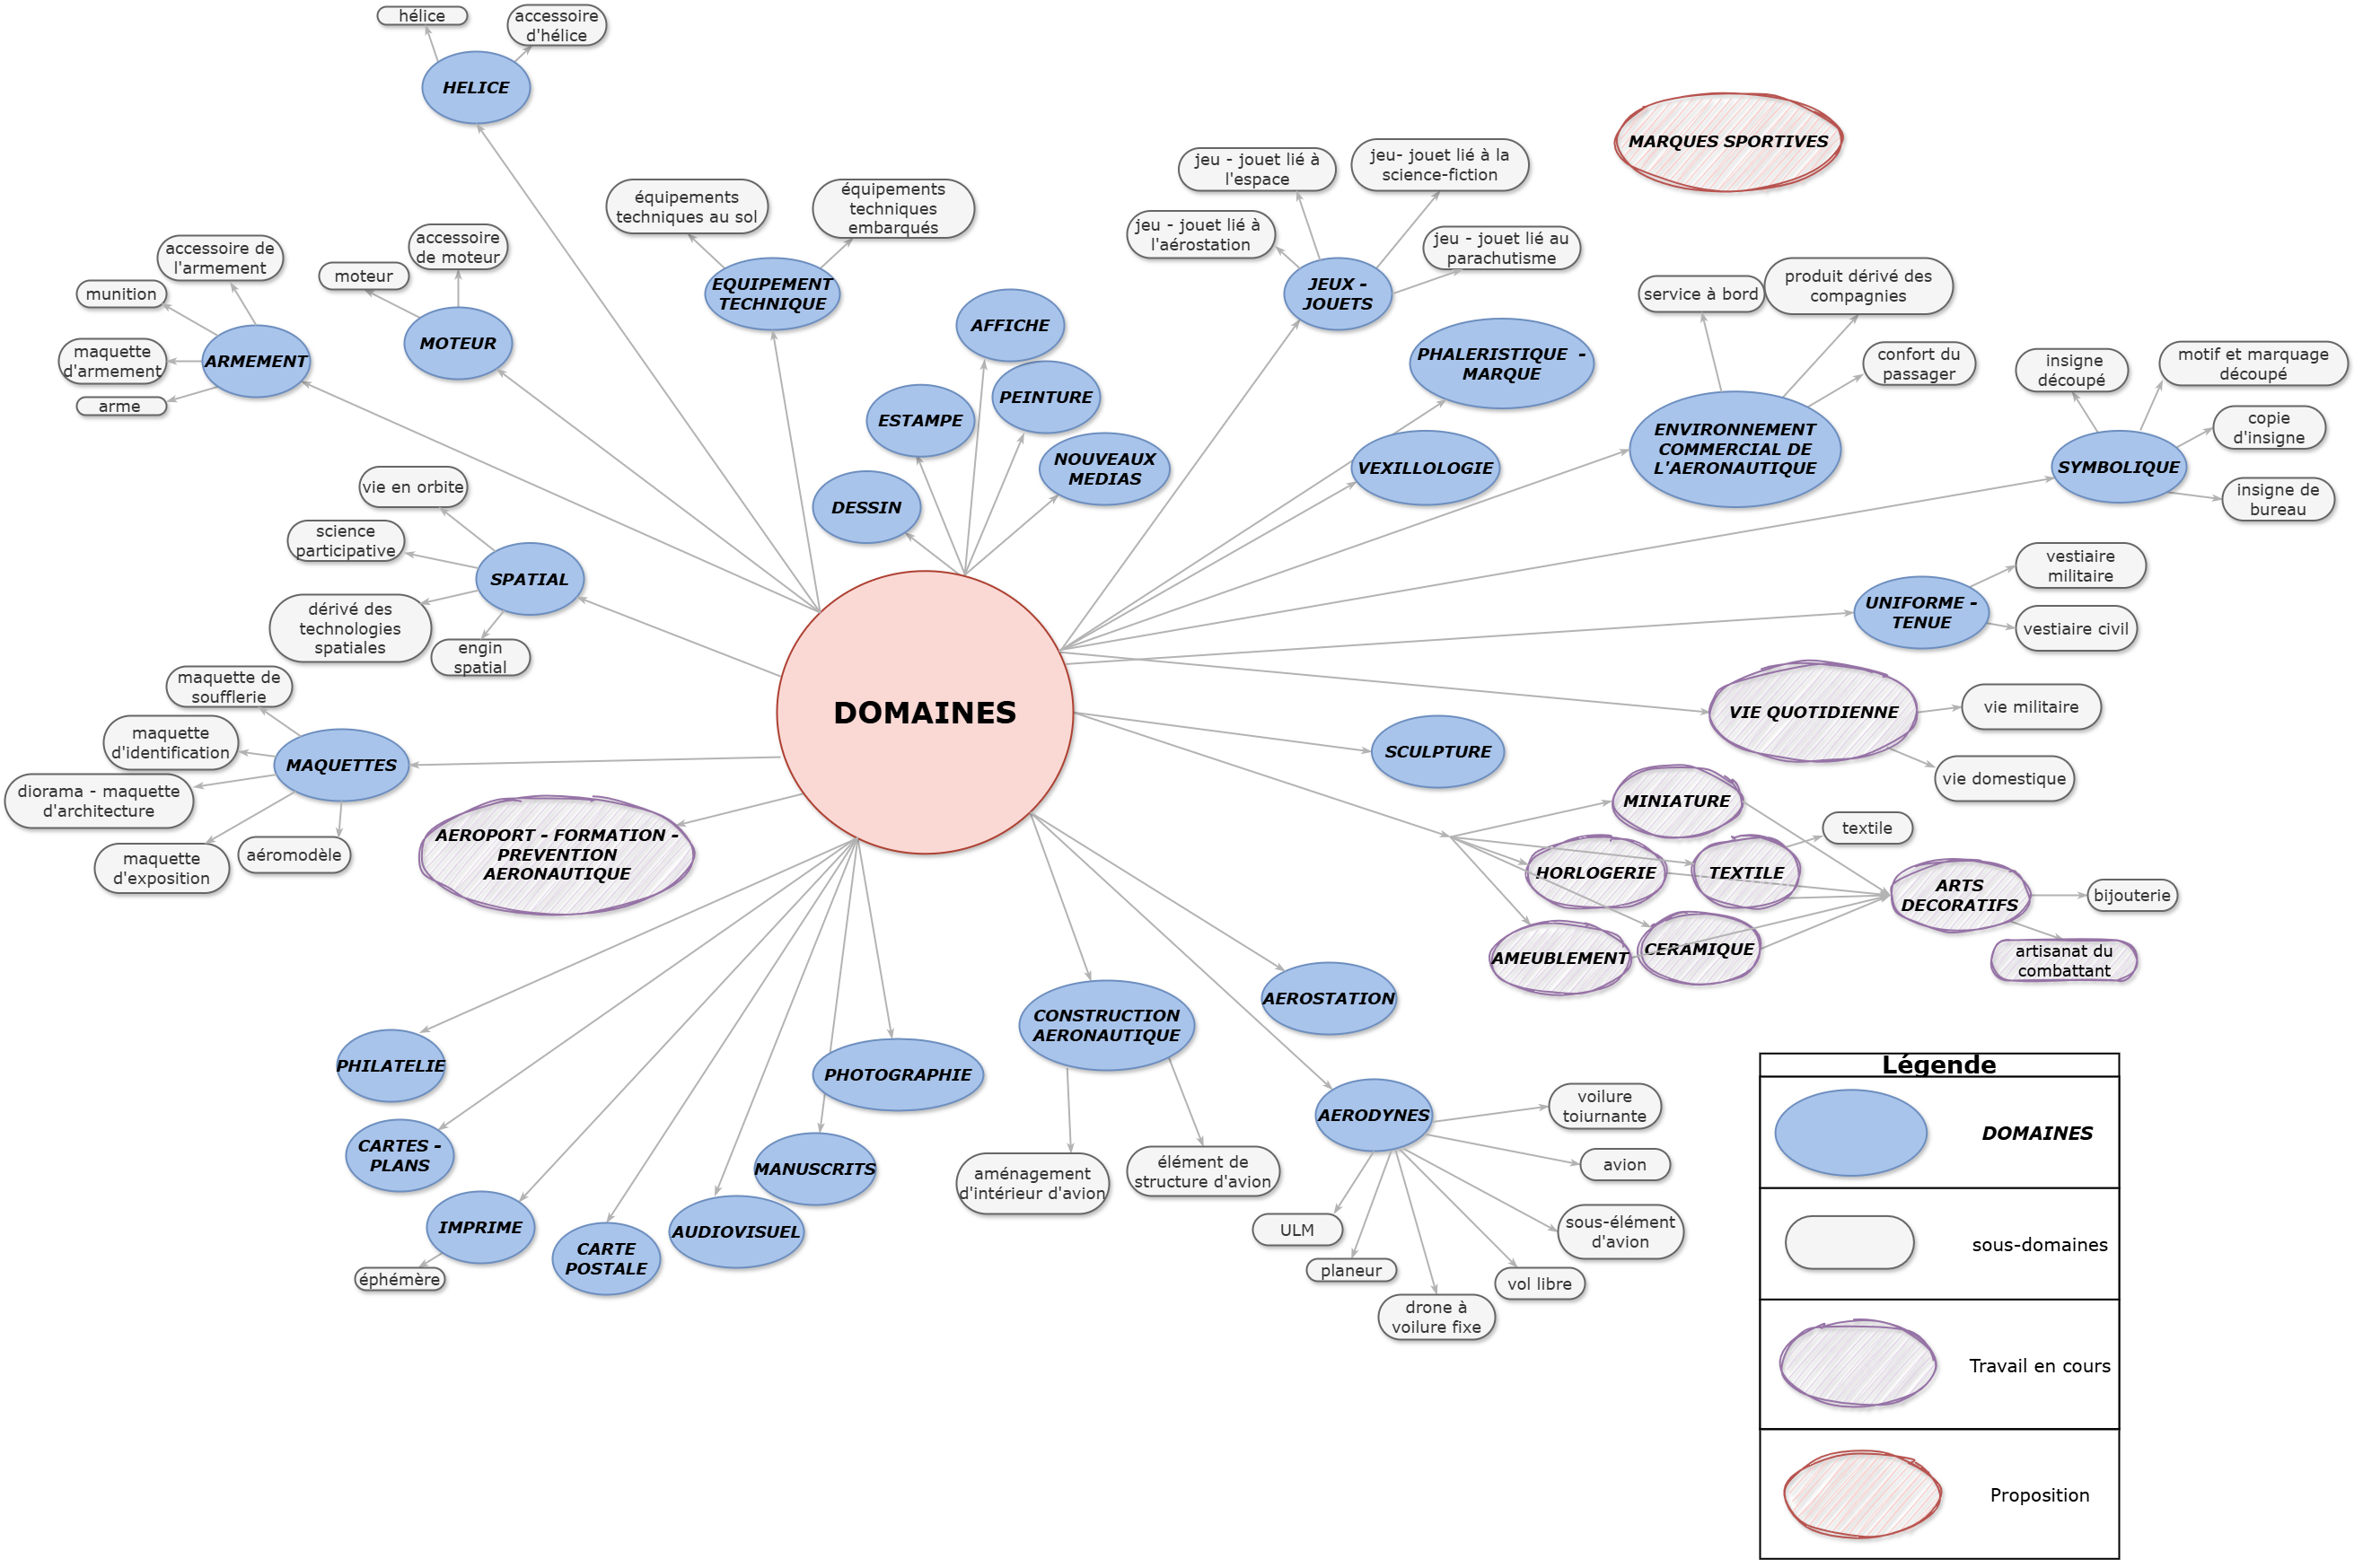
\includegraphics[width=\linewidth]{img/MODEL_domaines.png}
	\caption{Modélisation du thésaurus des domaines utilisés par le \mae}
	\label{fig:model_domaines}
\end{figure}

Le \mae incarne donc des défis propres aux musées techniques, bien différents de ceux des musées de beaux-arts et qui imposent des compétences croisées à la fois techniques et muséales. Les jeunes chargés de collections sont ainsi souvent issus de formations spécialisés — comme les masters du Muséum d’histoire naturelle — et passent par des institutions techniques ou militaires, telles que le musée de la Marine, le musée de l’Armée ou le \ac{cnam}. Ces musées doivent sans cesse composer avec des objets singuliers, souvent massifs, complexes à restaurer et à exposer.

Ces multiples défis sont rappelés par Agnès Mirambet-Paris et François Mirambet : diversité des matériaux, état de dégradation, inadéquation des environnements de conservation, échelle des objets, lourdeur des procédures, et besoin de ressources spécialisées\footcite{mirambet-parisConservationrestaurationPatrimoineTechnique2011}. Ils insistent sur la nécessité du dialogue entre techniciens et restaurateurs :
\begin{quote}
	\og C’est bien par le partage de compétences techniques acquises dans le domaine industriel et celles obtenues dans les écoles de formation à la restauration que pourront se développer pleinement des travaux de restauration\footcite{mirambet-parisConservationrestaurationPatrimoineTechnique2011}.\fg
\end{quote}

Le \mae incarne cette articulation entre expertise technique et exigence muséale. Ses pièces emblématiques — comme le Concorde 001 ou le scaphandre de Jean-Loup Chrétien\footcite{champenoisTresorsMuseeLair} — en font une institution unique, au croisement des enjeux de représentation nationale, de préservation patrimoniale et d’innovation culturelle.
